\documentclass{entcs}
\usepackage{entcsmacro}
\usepackage{z-eves}
\usepackage{graphicx}
\usepackage{url}

% The following is enclosed to allow easy detection of differences in
% ascii coding.
% Upper-case    A B C D E F G H I J K L M N O P Q R S T U V W X Y Z
% Lower-case    a b c d e f g h i j k l m n o p q r s t u v w x y z
% Digits        0 1 2 3 4 5 6 7 8 9
% Exclamation   !           Double quote "          Hash (number) #
% Dollar        $           Percent      %          Ampersand     &
% Acute accent  '           Left paren   (          Right paren   )
% Asterisk      *           Plus         +          Comma         ,
% Minus         -           Point        .          Solidus       /
% Colon         :           Semicolon    ;          Less than     <
% Equals        =3D           Greater than >          Question mark ?
% At            @           Left bracket [          Backslash     \
% Right bracket ]           Circumflex   ^          Underscore    _
% Grave accent  `           Left brace   {          Vertical bar  |
% Right brace   }           Tilde        ~

% A couple of exemplary definitions:

\newcommand{\Nat}{{\mathbb N}}
\newcommand{\Real}{{\mathbb R}}
\def\lastname{Lee}
\begin{document}
\begin{frontmatter}
  \title{A Z Approach in Validating ORA-SS Data Models}
  \author{Scott Uk-Jin Lee\thanksref{slee180@ec.auckland.ac.nz}}
  \author{Jing Sun\thanksref{j.sun@cs.auckland.ac.nz}}
  \author{Gillian Dobbie\thanksref{gill@cs.auckland.ac.nz}}
  \address{Department of Computer Science\\The University of Auckland\\
    Auckland, New Zealand}
  \author{Yuan Fang Li\thanksref{liyf@comp.nus.edu.sg}}
  \address{School of Computing\\National University of Singapore\\
    Singapore, Republic of Singapore}
  %\thanks[ALL]{Thanks to everyone who should be thanked}
  \thanks[slee180@ec.auckland.ac.nz]{Email:
    \href{mailto:slee180@ec.auckland.ac.nz} {\texttt{\normalshape
        slee180@ec.auckland.ac.nz}}}
  \thanks[j.sun@cs.auckland.ac.nz]{Email:
    \href{mailto:j.sun@cs.auckland.ac.nz} {\texttt{\normalshape
        j.sun@cs.auckland.ac.nz}}}
  \thanks[gill@cs.auckland.ac.nz]{Email:
    \href{gill@cs.auckland.ac.nz} {\texttt{\normalshape
        gill@cs.auckland.ac.nz}}}
  \thanks[liyf@comp.nus.edu.sg]{Email:
    \href{mailto:liyf@comp.nus.edu.sg} {\texttt{\normalshape
        liyf@comp.nus.edu.sg}}}
\begin{abstract}
  The rapid growth of the World Wide Web has resulted in more data
being accessed over the Internet. In turn there is an increase in
the use of semistructured data, which plays a crucial role in many
web applications particularly with the introduction of XML and its
related technologies. This increase in use makes the design of
good semistructured data structures essential. The Object
Relationship Attribute model for Semistructured data (ORA-SS) is a
graphical notation for designing and representing semistructured
data. In this paper, we demonstrate an approach to formally
validate the ORA-SS data models in order to enhance the
correctness of semistructured data design. A mathematical
semantics for the ORA-SS notation is defined using the Z formal
language, and further validation processes are carried out to
check the correctness of the semistructured data models at both
the schema and instance levels.
\end{abstract}
\begin{keyword}
  Semistructured data, ORA-SS data model, Formal specification and
  verification, Z specification language.
\end{keyword}
\end{frontmatter}

\section{Introduction}\label{intro}
The rapid growth of the World Wide Web and its technologies has
resulted in enormous amounts of data being used over the Internet
by Web Services and other Web-based applications. Many of the
applications use semistructured data, which is commonly
represented by eXtensible Markup Language (XML)~\cite{xml} and its
related technologies. With the growth in use of semistructured
data, the design of good semistructured data structures is
essential, particularly if the data is stored in a
database~\cite{wu01}. In order for the design and use of
semistructured data to be effective and efficient, it is very
important to have a good schema definition for semistructured
data. The Object Relationship Attribute model for Semistructured
data (ORA-SS) data modeling langauge~\cite{dobbie01orass} was
introduced for this purpose. For ORA-SS to be utilised widely, it
is essential to define a formal mathematical semantics for ORA-SS
since the current representation of ORA-SS is restricted to a
diagrammatic notation and semantics written in English. The
benefits of having such a formal semantics include:
\begin{itemize}
\item remove ambiguity that may arise from a diagrammatic
representation, \item enable the use of ORA-SS in other
applications and tools, and \item reveal inconsistencies in a
design at the schema and instance levels.
\end{itemize}
Inconsistencies at the schema level arise if a customized ORA-SS
schema model does not conform to the ORA-SS notation.
Inconsistencies at the instance level arise if an XML document is
not consistent with its schema. For example, an inconsistency that
might arise at the schema level is the specification of a ternary
relationship between only two object classes. An inconsistency
that might arise at the instance level is a many to many
relationship between elements when a one to many relationship is
specified in the schema. These two aspects of validation are
essential in the semistructured data design process. Thus, the
provision of formal semantics and reasoning support for validating
ORA-SS semistructured data modeling is very beneficial.
Furthermore, this validation also improves the quality
of applications utilizing semistructured data% by validating
%the instances of semistructured data such as XML against its
%schema
. Traditional validation of semistructured data is limited to
syntax checking only, e.g., XML Schema or DTD. However, deep
semantic checking and reasoning adds to the validation of
semistructured data design. The quality of the software system
will surely improve when these validation tasks are available for
applications which use semistructured data because methods of
ensuring correctness have expanded from plain syntax checking to
semantics checking.

In this paper, we demonstrate an approach to formally validate the
ORA-SS data models in order to enhance the correctness of
semistructured data design. Firstly, a mathematical semantics for
the ORA-SS diagrammatic notation is defined using the
Z~\cite{spi92a} formal language. Secondly we show how the
mathematical semantics is used in both the schema level and
instance level validation.
%
%Z is a specification language based on set theory and
%first-order predicate logic. It has been widely used for providing
%formal semantics and verifications in various application domains.
%In our previous work, we have applied Z and its proof tool in the
%verification of semantic web ontology models~\cite{dong04}.
There is related work using multimodal logic~\cite{bidoit04} and
spatial tree logic~\cite{ConfortiG03} to present and reason about
semistructured data. And a description logic representation of XML
documents can be found in \cite{calvanese99representing}. While
this work has helped us define the semantics of ORA-SS, there is
no promise of automated reasoning being applied to any of it at
the moment.

%The kind of verification introduced in this paper is very beneficial to
%any application using
%semistructured data, e.g., XML documents since the data used in
%the application can be validated formally. Instance level
%validation improves the quality of many applications utilizing
%semistructured data by validating the instances of semistructured
%data such as XML against its schema. Traditional verification for
%instances of semistructured data is limited to syntax checking
%only. However, deep semantic verification and reasoning can
%provide further enhancement of validating semistructured data
%design.
%%
%%The Z representation of ORA-SS and its verification can detect the
%%semantic incorrectness of semistructured data and its schema,
%%allowing the problems of the data to be fixed before its
%%utilization. This is a great benefit to the applications utilizing
%%semistructured data.
%The quality of the software system will surely increase when these
%verifications are available for applications which use
%semistructured data because methods of ensuring correctness have
%expanded from plain syntax checking to semantics checking. The Z
%representation and the verification can also be used in many
%industrial applications that use semistructured data. The back-end
%application can be developed using Z representation and
%verification. Then this back-end application can be used to verify
%the correctness of schemas and instances of semistructured data by
%connecting the developed verification application with DBMS (Data
%Base Management System) of industrial applications. This is very
%beneficial in improving the quality of industrial applications by
%assuring the correctness of the data used.

The rest of the paper is organized as follows. Section 2 presents
the background knowledge on ORA-SS notation and the Z formal
language. Section 3 presents a formal semantics of the ORA-SS
language in Z first-order logic. In Section 4, we demonstrate the
reasoning process of validating semistructured data models on both
an ORA-SS schema diagram and its XML instance. Section 5 concludes
the paper and describes future work.

\section{Background}
\subsection{ORA-SS data modeling language}
The Object Relationship Attribute model for Semistructured data
(ORA-SS) data modeling language~\cite{dobbie01orass,ling05}
consists of four basic concepts: object class, relationship type,
attribute and reference. It represents these concepts through four
diagrams: schema diagram, instance diagram, functional dependency
diagram and inheritance diagram.
\begin{itemize}
 \item An object class is like an entity
type in an ER diagram, a class in an object-oriented diagram or an
element in an XML document. The object classes are represented as
labelled rectangles in an ORA-SS diagram.
 \item A relationship type represents a nesting relationship among
object classes. It is represented optionally with a labelled
diamond and can be described by \texttt{name}, \texttt{n},
\texttt{p} and \texttt{c}. The \texttt{name} denotes the name of
relationship type, integer \texttt{n} indicates degree of
relationship type, \texttt{p} represents participation constraint
of parent object class in relationship type and \texttt{c}
represents participation constraint of child object class in
relationship type. The constraints are represented using
\texttt{min:max} notations with abbreviated symbols.
 \item  Attributes represent properties and are denoted by labelled circles.
An attribute can be a key attribute which has a unique value and
represented as a filled circle. An attribute can be a property of
an object or a property of a relationship. An attribute of an
object class has no label on its incoming edge and an attribute of
a relationship has the name of the associated relationship type on
its incoming edge.
 \item An object class can reference another object class
to model recursive and symmetric relationships, or to reduce
redundancy especially for many-to-many relationships. It is
represented by a labelled dashed edge. Disjunction of objects and
attributes is another thing that can be represented.
\end{itemize}
%For the representation of semistructured data, a schema
%diagram is derived from the instance where an instance is
%represented in an instance diagram. The functional dependency
%diagram in ORA-SS describes dependencies between data.
%It is often used in identifying redundancy in a
%resulting document. The inheritance diagram shows common
%properties of objects and helps data storage organization.
\begin{figure}[ht]
  \centering
  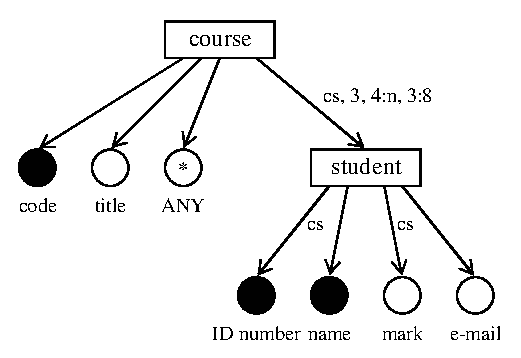
\includegraphics[width=76mm]{schema.eps}
  \caption{An example of an invalid ORA-SS schema diagram.}
  \label{schema}
\end{figure}
For example, Figure~\ref{schema} presents an ORA-SS schema that
represents the structure of a particular semistructured data.
%is syntactically correct but semantically wrong.
This schema diagram shows that there is a relationship between the
`\texttt{course}' object class and the `\texttt{student}' object
class, and this relationship has a single-valued attribute
`\texttt{mark}'. The object class `\texttt{course}' has an
identifier `\texttt{code}', with single-valued attribute
`\texttt{title}' and multi-valued attribute `\texttt{ANY}'. Object
class `\texttt{student}' has identifier `\texttt{ID number}', and
single valued attributes `\texttt{name}' and `\texttt{email}'.
However, the above schema diagram is syntactically correct but
there are three semantic errors. The degree of relationship
`\texttt{cs}' is 3, representing a ternary relationship where it
actually is a binary relationship since object `\texttt{course}'
is not related to any other objects besides `\texttt{students}'.
Another semantic error is having two primary keys for the object
class `\texttt{student}'. There are two attributes selected as
primary key where there should only be one primary key for each
object class. The third semantic error in this schema is that the
primary key `\texttt{ID number}' is represented as an attribute of
the relationship `\texttt{cs}' where it really is an attribute of
an object `\texttt{student}'. A validation process should pick up
this kind of errors in the design.

\subsection{Z formal specification langauge}

Z~\cite{wood96} is a formal specification language originally
developed at the Programming Research Group at Oxford University
and it is probably the most popular formal specification language
currently available. It is based on set theory and first-order
predicate logic. Z is a declarative language and it has a number
of language constructs including given type, abbreviation type,
axiomatic definition, state and operation schema definitions. It
has been widely used for providing formal semantics and
verifications in various
application domains. %
%
%Among these many language constructs, schema definitions are often
%used in Z to describe a system~\cite{spi92a}. Z uses schema
%definitions derived from mathematics to state real world problems,
%to discover solutions and to prove that the chosen design meets
%the specification. The schema definition encapsulates declarations
%of fixed sets and variables as well as the specification of a
%relationship between them represented through predicates. %In a Z
%%formal specification, schema definitions are categorised into
%%either state schemas or operation schemas. A state schema is used
%%to describe the state of the system where an operation schema is
%%used to describe state changes by expressing a relationship
%%between values of variables before and after the operation. These
%%two schemas are both used to describe the system properties.
%The schema definitions allow Z to facilitate composition of
%complex specifications. With schema definitions Z provides a
%simple, precise, mathematical language for description and
%communication. Also there are many tools available to support its
%use.
Z/EVES~\cite{saaltink97zeves} is an interactive system for
composing, checking, and analyzing Z specifications. In
particular, it supports general theorem proving of Z
specifications.
%

\section{Formal semantics of ORA-SS data modeling langauge}
%
\subsection{Basic types}
Initially basic types used in the ORA-SS data modeling language
must be identified and defined prior to constructing the formal
representation. %In the ORA-SS data modeling language, object
%classes and attributes are the basic types required for providing
%a schema definition of semistructured data.
\begin{small}
\begin{zed}
  [OBJCLASS, OBJECT, ATTRIBUTE, ATTVALUE]\\
\end{zed}
\end{small}
The object types and attribute types defined above represent the
set of object classes, object instances, attributes and attribute
values respectively in the ORA-SS language. %`\texttt{OBJCLASS}' and `\texttt{ATTRIBUTE}'
%types are required to define schema representations and general
%semantics of ORA-SS data modeling language such as relationships,
%attributes of objects and relationships, and so on. The
%`\texttt{OBJECT}', `\texttt{ATTVALUE}' types which refer to object
%instances and attribute values respectively, are required for
%representing the semantics of ORA-SS instance data that requires
%constraints on the XML instance such as participation constraints
%of relationships, cardinality on attribute values and so on.
%\begin{small}
%\begin{sidebyside}[4]
%\begin{axdef}
%  zero: \nat
%\where
%  zero = 0
%\end{axdef}
%\nextside
%\begin{axdef}
%  one: \nat
%\where
%  one = 1
%\end{axdef}
%\nextside
%\begin{axdef}
%  number: \nat
%\where
%  number \geq  2
%\end{axdef}
%\nextside
%\begin{axdef}
%  many: \nat
%\where
%  \forall  n: \nat  @ many > n
%\end{axdef}
%\end{sidebyside}
%\end{small}

%A additional type `MULTIPLICITY' is defined as a collection of
%definitions for all possible multiplicity values. In the ORA-SS
%data modeling language, multiplicity values are used for
%specifying the number of participation of objects in relationship
%type or cardinalities of attribute values associated with an
%object.
%\begin{small}
%\begin{zed}
%MULTIPLICITY == \{zero, one, number, many\}
%\end{zed}
%\end{small}
%In the ORA-SS data modeling language multiplicities used for
%participation constraints are specified using two different
%notations, natural numbers and symbols with its own meaning.
%Multiplicities `\texttt{0}' and `\texttt{1}' are specified as
%natural numbers and multiplicities `\texttt{n}' and `\texttt{m}'
%are specified as symbols that stands for any number and many
%respectively.
%The different notations used for multiplicities in
%ORA-SS data model language does not allow the multiplicities to be
%represented as single type such as `N' natural number, resulting a
%construction of new ways to represent the multiplicities in a
%single type. The above type definition called `MULTIPLICITY'
%represented the multiplicity in a single type by defining each
%multiplicity separately and set it as `MULTIPLICITY' type. The
%multiplicity `0', `1' and `n' is defined exactly as it is where
%all of them are natural numbers 0, 1 and natural number larger
%than 2 respectively but the multiplicity `m' is defined slightly
%different. Since the multiplicity `m' represents infinity it is
%defined as natural number which is larger than n where n is any
%natural number. The definition of multiplicity `m' certainly
%represents infinity because natural number larger than all the
%natural number can be considered as infinity. The multiplicity
%type definition constructed can now be used in other definitions
%for formal semantics of ORA-SS data model language since all
%possible multiplicities are represented as a `MULTIPLICITY' type.

\subsection{Relationship type}
Relationship type is defined as a function with a set of object
classes as its domain and a sequence of set of object classes as
its range. The predicate of the function uses a recursive
definition and describes that object classes can be related to
other object classes as well as to other relationships.
\begin{small}
\begin{axdef}
  relationship: \power OBJCLASS \fun \seq _1{} (\power OBJCLASS)
\where
  \forall objclses: \power OBJCLASS; seqobjclses: \seq _1{} (\power OBJCLASS) \\
  \t1 @  \{objclses \mapsto  seqobjclses\} \subset  relationship \\
  \t1  \iff (\forall  objclses0: \ran  seqobjclses @ objclses \cap  objclses0 = \emptyset) \\
  \t2 \land  (\# seqobjclses = 1 \\
  \t3 \lor  (\# seqobjclses \geq  2 \\
  \t4 \implies  \{head~seqobjclses \mapsto  tail~seqobjclses\} \subset relationship))
\end{axdef}
\end{small}
In an ORA-SS schema diagram, there are two types of relationship,
i.e., a normal relationship where the child participant is a
single object class; and a disjunctive relationship where the
child participant is a set of disjunctive object classes. The
above definition includes both cases. It defines a relationship as
a function where the first argument represents the child object
classes in a relationship and the second argument represents a
sequence of set of object classes which refers to either a parent
object class or another sub-relationship. Note that the `$\power
OBJCLASS$' denotes both the normal relationship case where the
child is a singleton object class set, and the disjunctive
relationship case where the child is a set of disjunctive object
classes.

The first predicate of the function defines that the child object
classes should not intersect with any of the object classes at the
parent level. This is to prevent cyclic definitions in the
relationship structure. The second predicate states that child
object classes can be connected to either a singleton sequence of
object classes which forms a binary relationship, or with a
sequence that has more than two elements which represents a
relationship of degree 3 or more. It specifies that when the
cardinality of the object classes sequence is greater or equal to
two, the head of the sequence and its tail forms another
sub-relationship type.

\subsection{Degree of a relationship type}
Every relationship in an ORA-SS schema diagram has its associated
degree represented as a natural number.
\begin{small}
\begin{axdef}
  degree: relationship \fun \nat _1{}
\where
  \forall  rel0: relationship @ degree~rel0 = \# (second~rel0) + 1
\end{axdef}
\end{small}
The above definition defines a degree as a function where the
first argument represents the relationship and the second argument
represents the natural number which refers to the value of the
degree of the relationship. The predicate of the function defines
that the degree of any relationship is 1 added to the cardinality
of the sequence of set of object classes which represents either a
parent object class or a sub-relationship. It basically specifies
the degree of a relationship is the number of object classes
involved in the relationship.

\subsection{Instances of object class and attribute}
In the ORA-SS data model, an object class has instances which are
objects.
\begin{small}
\begin{axdef}
  hasObjInstance: OBJCLASS \fun  \power  OBJECT
\where
  \forall  object1, object2: OBJCLASS @ object1 \neq  object2 \\
  \t1 \implies  hasObjInstance~ object1 \cap  hasObjInstance~ object2 = \emptyset
\end{axdef}
\end{small}
The above definition defines object classes having instances as a
function. In this function, the first argument represents an
object class and the second argument represents a set of objects
which refers to all the instances of the object class. The
predicate of the function defines that any two different object
classes should have different object instances. This specifies
that an object cannot be an instance of multiple object classes.
As an object class has instances, attributes also have values. A
similar definition can be provided.

\subsection{Instances of a relationship type}
In the ORA-SS data model, a relationship type also has its
instances which represents the participation instances from their
corresponding object classes in the relationship.
\begin{small}
\begin{axdef}
  hasRelInstance: relationship \fun  (OBJECT \rel  \seq _1{}
  OBJECT)
\where
  \forall  rel0: relationship; relinsts0: OBJECT \rel  \seq _1{} OBJECT \\
  @ relinsts0 = hasRelInstance~ rel0 \\
  \iff  (\forall  relinst: relinsts0 \\
  \t1 @ \# (second~ relinst) + 1 = degree~ rel0 \\
  \t1 \land  (\exists _1{} objcls: first~ rel0 @ \\
  \t2 \dom  (relinsts0 \rres  \{second~ relinst\}) \subseteq  hasObjInstance~ objcls) \\
  \t1 \land  ((\# (second~ relinst) = 1 \\
  \t2 \implies  \# (second~ rel0) = 1 \\
  \t3 \land  (\exists _1{} objcls: head (second~ rel0) \\
  \t4 @ head (second~ relinst) \in  hasObjInstance~ objcls)) \\
  \t1 \lor  (\# (second~ relinst) \geq  2 \\
  \t2 \implies  (head (second~ relinst), tail (second~ relinst)) \\
  \t3 \in  hasRelInstance (head (second~ rel0) \mapsto  tail (second~ rel0)))))\\
  \forall  rel1, rel2: relationship | rel1 \neq  rel2 \\
  \t1 @ hasRelInstance~ rel1 \cap  hasRelInstance~ rel2 = \emptyset
\end{axdef}
\end{small}
The above definition defines relationship having instances as a
function where the first argument represents a relationship and
the second argument represents the instance of the relationship.
An instance of the relationship is represented as an object
related to a sequence of objects that conforms to the relationship
definition.

The first predicate of the function defines that the degree of a
relationship instance should be the same as the degree of the
relationship type. The second predicate defines that child object
instance should be an instance of the associated selected child
object classes in the relationship. Also the predicate defines
that only the objects of a single object class is related to a
parent object or sub-relationship instance in the case of a
disjunctive relationship. The third predicate consists of two
cases. If the degree of the relationship is binary, the parent
object instance should be an instance of the parent object class.
If the degree of the relationship is ternary or more, the second
part of the predicate recursively defines that the
sub-relationship instance sequence is an instance of the
sub-relationship type. Finally, the last predicate defines that
any two relationship types should have their own disjoint set of
instances. This is to specify that a relationship instance cannot
be an instance of multiple relationship types.

\subsection{Participation constraints on objects in a relationship type}
Every relationship type in an ORA-SS schema diagram has its
associated constraints on its participating objects which is
represented by the `\texttt{min:max}' notation. It constrains the
number of child objects that a parent object can relate to and
vice versa.
\begin{small}
\begin{axdef}
  parentConstraints: relationship \fun (MULTIPLICITY \cross MULTIPLICITY)
  \where
  \forall  rel0: relationship; card: (MULTIPLICITY \cross  MULTIPLICITY) \\
  \t1 @ parentConstraints~ rel0 = card \\
  \t1 \iff  (\# (second~ rel0) < 2 \\
  \t2 \implies  (\forall  obj: OBJECT \\
  \t3 | (\exists _1{} objcls: head~ (second~ rel0) @ obj \in  hasObjInstance~ objcls) \\
  \t3 @ card.1 \leq  \# ((hasRelInstance~ rel0) \rres  \{\langle obj\rangle \}) \leq card.2)) \\
  \t1 \land  (\# (second~ rel0) \geq  2 \\
  \t2 \implies  (\forall  subrelinst: hasRelInstance~ (head~ (second~ rel0) \\
  \t9 \mapsto  tail~ (second~ rel0)) \\
  \t3 @ card.1 \leq  \# ((hasRelInstance~ rel0) \\
  \t4 \rres  \{(\langle first~ subrelinst\rangle  \cat  second~ subrelinst)\}) \leq  card.2))
\end{axdef}
\end{small}
The above definition defines parent constraints as a function
where the first argument represents a relationship and the second
argument represents a cartesian product of multiplicity which
refers to a `\texttt{min:max}' pair. The predicate of the function
defines that the number of relationship instances in which each
object of the parent object class or each relationship instance of
the sub-relationship type should be within the multiplicities
defined in the relationship. It specifies that the parent
constraint sets the boundaries for the number of child objects
that a single parent object or sub-relationship instance can have.
The child constraints of the relationship can be defined in a
similar way.


\subsection{Object class, attribute pairs and their instances}
In ORA-SS schema diagrams, an object can have a set of attributes.
\begin{small}
\begin{axdef}
  hasObjectAttribute: OBJCLASS \fun  \power  ATTRIBUTE
\end{axdef}
\end{small}
The association between attributes and an object class also has a
set of instances, which is defined in the definition
`\texttt{hasObjAttrInstance}'.
\begin{small}
\begin{axdef}
  hasObjAttrInstance: hasObjectAttribute \fun  (OBJECT \rel  \power
  ATTVALUE)
\where
  \forall  objattr: hasObjectAttribute; objattrinsts: (OBJECT \rel  \power  ATTVALUE)\\
  \t1 @ hasObjAttrInstance~ objattr = objattrinsts \\
  \t1 \iff  (\forall  objattrinst0: objattrinsts \\
  \t2 @ (first~ objattrinst0) \in  hasObjInstance (first~ objattr) \\
  \t2 \land  \# (second~ objattrinst0) = \# (second~ objattr) \\
  \t2 \land  (\forall  attrVal: second~ objattrinst0 \\
  \t3 @ (\exists _1{} attr: second~ objattr @ attrVal \in  hasAttValue~ attr)) \\
  \t2 \land  (\forall  attr: second~ objattr
   @ (\exists _1{} attrVal: second~ objattrinst0 \\
  \t3 @ attrVal \in  hasAttValue~ attr)))
\end{axdef}
\end{small}
The first argument represents `hasObjectAttribute' function and
the second argument represents a set of pair of an object and set
of attribute values. The first two predicates define that for all
the objects and attribute value sets, the object should belong to
the object class in the `\texttt{hasObjectAttribute}' function and
the cardinality of the attribute value set should be the same as
the cardinality of the attribute in the
`\texttt{hasObjectAttribute}' function. The third and fourth
predicates define that each attribute value should belong to one
and only one corresponding attribute specified in
`\texttt{hasObjectAttribute}' function and vice versa. Attributes
can belong to relationships and relationship attributes have their
own instances. The relationship attributes and their instance can
be defined similarly.

\subsection{Candidate key and primary key of an object class}
An object can have an attribute or set of attributes that have a
unique value for each instance of an object class called a
candidate key. There are two types of candidate key, i.e., a
candidate key where the key is a single attribute; and a composite
candidate key where the key is a set of attributes. The following
definition includes both cases.
\begin{small}
\begin{axdef}
  hasObjectCandidateKey: OBJCLASS \rel  \power  ATTRIBUTE
\where
  \forall  object0: OBJCLASS; key0: \power  ATTRIBUTE \\
  @ (object0, key0) \in  hasObjectCandidateKey \\
  \iff  key0 \subseteq  hasObjectAttribute~ object0 \\
  \t1 \land  (\forall  keyValue1, keyValue2: \power  ATTVALUE;\\
  \t2 objInst1, objInst2: hasObjInstance~ object0\\
  \t2 | (\forall  attrVals1: \ran  (\{objInst1\} \\
  \t3 \dres  hasObjAttrInstance (object0, (hasObjectAttribute~
  object0)))\\
  \t3 @ keyValue1 \subseteq  attrVals1) \\
  \t2 \land  (\forall  attrVals2: \ran  (\{objInst2\} \\
  \t3 \dres  hasObjAttrInstance (object0, (hasObjectAttribute~ object0))) \\
  \t3 @ keyValue2 \subseteq  attrVals2) \\
  \t2 @ ((keyValue1 \neq  keyValue2 \implies  objInst1 \neq
  objInst2)\\
  \t3 \land  (keyValue1 = keyValue2 \implies  objInst1 = objInst2)))
\end{axdef}
\end{small}
It defines the object having a candidate key as a relationship
where object classes are related to the set of attributes which
refer to all the candidate keys that belong to the object. Note
that the `\texttt{$\power$ ATTRIBUTE}' denotes both a candidate
key and a composite candidate key. The first predicate of the
function defines that candidate keys belong to the set of
attributes that the object has. The second predicate of the
function defines two facts. It states that two objects are
different when values of the candidate key for each object are
different; and two objects are the same when values of the
candidate key for each object are the same, where the values of
the candidate keys belongs to the set of attribute values of the
object attributes. This specifies that the value of candidate key
for each object of an object class should uniquely identify an
object instance.
\begin{small}
\begin{axdef}
  hasObjectPrimaryKey: OBJCLASS \fun  \power  ATTRIBUTE
\where
  hasObjectPrimaryKey \subseteq  hasObjectCandidateKey
\end{axdef}
\end{small}
In ORA-SS schema diagrams, an object class has a primary key which
is selected from the set of candidate keys. The
`\texttt{hasObjectPrimaryKey}' is defined as a total function type
which indicates each object class can relate to one and only one
set of attributes as its primary key.

%where the first argument is an object class and the second
%argument is a set of attributes which is the primary key. The
%predicate of the function states that this function is a subset of
%`\texttt{hasObjectCandidateKey}' relation since primary key is a
%chosen candidate key. Note the `\texttt{hasObjectPrimaryKey}' is
%defined as a total function type which indicates each object class
%can relate to one and only one set of attributes as its primary
%key.
%
%\subsection{Disjunctive attribute and its values}
%
%Disjunctive attribute is another kind of attribute in ORA-SS
%schema diagram, whose value can be selected from a set of
%disjunctive attributes.
%
%\begin{axdef}
%  disjunctiveAttribute: ATTRIBUTE \pfun  \power  ATTRIBUTE
%\where
%  \forall  disjAtt0: \dom  disjunctiveAttribute @ \# (disjunctiveAttribute~ disjAtt0) \geq  2
%\end{axdef}
%
%The above defines the disjunctive attribute where the first
%argument is attribute and the second argument is set of
%attributes. The predicate of the function states that disjunctive
%attribute should have two or more attributes to choose from. A
%disjunctive attribute also has its values. It can be defined as
%follows.
%
%\begin{axdef}
%  hasDisjunctiveAttValue: disjunctiveAttribute \fun  (ATTVALUE \rel
%  ATTVALUE)
%\where
%  \forall  disjuncAtt0: disjunctiveAttribute; disjuncAttVals: ATTVALUE \rel  ATTVALUE \\
%  @ hasDisjunctiveAttValue~ disjuncAtt0 = disjuncAttVals \\
%  \iff  (\forall  attValpair: disjuncAttVals \\
%  \t1 @ first~ attValpair \in  hasAttValue (first~ disjuncAtt0)\\
%  \t2 \land  (\exists _1{} att: second~ disjuncAtt0 \\
%  \t3 @ \ran  (\{first~ attValpair\} \dres  disjuncAttVals) \subseteq  hasAttValue~ att))
%\end{axdef}
%
%The above definition defines disjunctive attribute having its
%value as a function where the first argument represents
%disjunctive attribute definition and the second argument
%represents the set of attribute value pairs which is attribute
%value of the parent of disjunctive attribute related to the
%attribute value of the child. The predicate of the function
%defines that for each attribute value pair, the first value should
%belong to the parent attribute and the second attribute value
%should be selected from one of the disjunctive child attributes.
%Similarly, we can give a definition for the composite attribute
%type and its values.
%
\subsection{Cardinality of attribute values associated with an object}
As a relationship type has its associated participation
constraints, attributes also has cardinality constraints
associated with an object instance. It constrains the number of
attribute values that an object can have.
\begin{small}
\begin{axdef}
  hasAttCardinality: ATTRIBUTE \fun  (MULTIPLICITY \cross
  MULTIPLICITY)
\where
  \forall  attr0: ATTRIBUTE; card: MULTIPLICITY \cross  MULTIPLICITY \\
  @ hasAttCardinality~ attr0 = card \\
  \iff  (\forall  obj: OBJCLASS | attr0 \in  hasObjectAttribute~ obj \\
  \t1 @ (\forall  objinst: hasObjInstance~ obj \\
  \t2 @ card.1 \leq  \# (\{objinst\} \\
  \t3 \dres  hasObjAttrInstance (obj, (hasObjectAttribute~ obj))) \\
  \t2 \leq  card.2)) \\
  \lor  (\forall  rel: relationship | attr0 \in  hasRelationshipAttribute~ rel \\
  \t1 @ (\forall  relinst: hasRelInstance~ rel \\
  \t2 @ card.1 \leq  \# (\{relinst\} \\
  \t3 \dres  hasRelAttrInstance (rel, (hasRelationshipAttribute~ rel))) \\
  \t2 \leq  card.2))
\end{axdef}
\end{small}
The above definition states the cardinality constraints of
attributes as a function where first argument represents attribute
and the second argument represent a cartesian product of
multiplicity which refers to the `\texttt{min:max}' form. The
predicate of the function defines that the number of attribute
values for each object or relationship instance should be within
the multiplicities specified on the attribute.
%
%In ORA-SS schema diagram, attributes can be single-valued,
%multi-valued, required or optional. These properties of the
%attributes depend on the cardinality constraint of the attribute.
%They can be defined as follows.
%
%\begin{sidebyside}[2]
%\begin{axdef}
%  isSingleValued: \power  ATTRIBUTE
%\where
%  \forall  attr: isSingleValued \\
% @ second (hasAttCardinality~ attr) \\
% \t1 = one
%\end{axdef}
%\nextside
%\begin{axdef}
%  isMultiValued: \power  ATTRIBUTE
%\where
%  \forall  attr: isMultiValued \\
%  @ second (hasAttCardinality~ attr) \\
%  \t1 = many
%\end{axdef}
%\end{sidebyside}
%\begin{sidebyside}
%\begin{axdef}
%  isRequired: \power  ATTRIBUTE
%\where
%  \forall  attr: isRequired \\
%  @ first (hasAttCardinality~ attr) \\
%  \t1 = one
%\end{axdef}
%\nextside
%\begin{axdef}
%  isOptional: \power  ATTRIBUTE
%\where
%  \forall  attr: isOptional \\
%   @ first (hasAttCardinality~ attr)\\
%   \t1 = zero
%\end{axdef}
%\end{sidebyside}
%
%The definition of `\texttt{isSingleValued}' states that the
%maximum cardinality of the attribute is `\texttt{one}'. This is to
%represent that single-valued attributes can have at most one
%value. The definition of `\texttt{isMultiValued}' states that the
%maximum cardinality of the attribute is `\texttt{many}'. This is
%to represent that multi-valued attributes can have many values.
%The definition of `\texttt{isRequired}' states that the minimum
%cardinality of the attribute is `\texttt{one}'. This is to
%represent that required attributes must have at least one value.
%The definition of `\texttt{isOptional}' states that the minimum
%cardinality of the attribute is `\texttt{zero}'. This is to
%represent that optional attributes can have its value or none.
%
In this section, we presented some of the formal semantics of the
ORA-SS language constructs using the Z first-order logic. Due to
the space limit, not all the semantic definitions are presented
here. Other ORA-SS constructs can be defined in a similar manner.

\section{Validating semistructured data}
%
As we mentioned earlier, a major concern in designing a good
semistructured data structure for a particular application is to
ensure there are no possible inconsistencies in either the ORA-SS
schema diagram or the XML instance. Having defined a formal
semantics of ORA-SS in Z, we can present and validate any ORA-SS
schema diagram and its XML instances.

\subsection{Schema diagram validation}
Schema validation involves checking whether a customized ORA-SS
schema diagram is consistent according to the semantics of the
ORA-SS language. Possible guidelines for validating an ORA-SS
schema diagram are as follows.
\begin{itemize}
 %relationship
 \item In a relationship type, the child object class must be either related to another
parent object class to form a binary relationship or related to
another sub-relationship type to form a relationship type of
degree 3 or more.
 \item The degree of a binary relationship is 2, ternary is 3 and
 n-nary is n.
 \item In a disjunctive relationship type, the child participants
is a set of disjunctive object classes.
 %attribute
 \item A composite attribute or disjunctive attribute has an attribute that is
 related to two or more sub-attributes.
 \item A candidate key of an object class is selected from the
 set of attributes of the object class.
 \item A composite key is selected from 2 or more attributes of an object class.
 \item There can only be one primary key per object class and it can be
either a candidate key or a composite candidate key.
 \item  Relationship attributes have to relate to an existing
relationship.
 %reference
 \item An object class can reference one object class only, but an
 object class can be referenced by multiple object classes.
\end{itemize}
The above are some of the criteria for validating a schema diagram
against the ORA-SS notation. As we can see from the previous
section, most of these guidelines have already been encoded into
the Z semantics of ORA-SS. Thus when we represent a particular
ORA-SS schema model in Z, we can validate the correctness of the
schema diagram against the ORA-SS Z semantics. For example, we can
represent the schema diagram in Figure~\ref{schema} and validate
it as follows.
\begin{small}
\begin{axdef}
  Course, Student: OBJCLASS\\
  Code, Title, Any, IDNumber, Name, Mark, EMail: ATTRIBUTE\\
  cs: relationship
\where
  hasObjectAttribute~ Course = \{Code, Title, Any\}\\
  hasObjectAttribute~ Student = \{Name, EMail\}\\
  cs = \{Student\} \mapsto  \langle \{Course\}\rangle \\
  degree~ cs = 3\\
  parentConstraints~ cs = (4, many)\\
  childConstraints~ cs = (3, 8)\\
  hasRelationshipAttribute~ cs = \{IDNumber, Mark\}\\
  hasObjectPrimaryKey~ Course = \{Code\}\\
  hasObjectPrimaryKey~ Student = \{IDNumber\}\\
  hasObjectPrimaryKey~ Student = \{Name\}
\end{axdef}
\end{small}
%The following shows some of the schema validation steps regarding
%the example above.
\begin{itemize}
    \item{\bf Validating the degree of the \texttt{cs} relationship}:
    \begin{small}
    \begin{zed}
      degree~ cs = degree (\{Student\} \mapsto  \langle
      \{Course\}\rangle) \\
       = \# (second (\{Student\} \mapsto  \langle
      \{Course\}\rangle) ) + 1 \\
      = \# (\langle
      \{Course\}\rangle) + 1 = 2 \neq 3\\
       \implies false
    \end{zed}
    \end{small}
    Thus the definition of $degree~ cs = 3$ is invalid.
    \item {\bf Validating the primary key of the \texttt{Student} object class}:
     \begin{small}
     \begin{zed}
      hasObjectPrimaryKey~ Student = \{IDNumber\} \\
      \implies
      Student \mapsto \{IDNumber\} \in hasObjectCandidateKey \\
       \implies \{IDNumber\} \subseteq hasObjectAttribute~Student\\
       \implies
      \{IDNumber\}\subseteq  \{Name, EMail\} \\
       \implies false
    \end{zed}
    \end{small}
     Thus the attribute `\texttt{IDNumber}' can not be a primary key of the
     `\texttt{Student}' object class since it is an attribute of the
     relationship `\texttt{cs}'.
      \begin{small}
      \begin{zed}
      hasObjectPrimaryKey~ Student = \{IDNumber\} \\
      \land hasObjectPrimaryKey~ Student =
      \{Name\}\\
       \implies \{Student \mapsto \{IDNumber\}, Student \mapsto \{Name\}\}
      \subseteq hasObjectPrimaryKey \\
       \land hasObjectPrimaryKey \subseteq OBJCLASS \fun \power
      ATTRIBUTE\\
       \implies false
    \end{zed}
    \end{small}
     Since `\texttt{hasPrimaryKey}' is defined as a function mapping from
     an object class to a set of attributes as its primary key, one object class in
     the domain can not be mapped to two different values in the range in a
     function definition. Thus the attribute `\texttt{IDNumber}' and
     `\texttt{Name}' can not both be the primary
     keys of the object class `\texttt{Student}'. Intuitively, we
     chose the `\texttt{IDNumber}' as the key since the
     `\texttt{Name}' may not uniquely identify a student object.
\end{itemize}
After revealing all the errors we can correct the ORA-SS schema
example in Figure~\ref{schema} by removing the `\texttt{name}'
attribute in the student as a primary key. %From above, we
%demonstrated some validation steps using a simple ORA-SS schema
%example. More complicated proof steps can be established in
%validating large schema data models to check the correctness of a
%semistructured data design.

\subsection{XML instance validation}
The XML instance validation is defined to check whether there are
any possible inconsistencies in a semistructured data instance,
where an XML document should be consistent with regard to the
designated ORA-SS schema diagram. Possible guidelines for
validating an XML instance are as follow.
\begin{itemize}
 \item Relationship instances must conform to the parent participation
constraints, e.g., the number of child objects related to a single
parent object or relationship instance should be consistent with
the parent participation constraints; and the number of parent
objects or relationship instances that a single child object
relates to should be consistent with the child participation
constraints.
 \item  In a disjunctive relationship, only one object class can be
 selected from the disjunctive object class set and associated to a
 particular parent instance.
 \item For a candidate key (single or composite), its value should
 uniquely identify the object that this key attribute belongs to.
 \item Each object can have one and only one primary key.
 \item All attributes have their own cardinality and the number of attributes
that belong to an object should be limited by the minimum and
maximum cardinality values of the attribute.
 \item For a set of disjunctive attributes, only one of the attribute choices
 can be selected and associated to an object instance.
\end{itemize}
These are some of the criteria of instance level validation. Given
an XML instance file, we should be able to check the consistency
of the content in the document against its ORA-SS schema
definitions.
%Because the ORA-SS schema model imposes constraints
%on the structure of its XML instance, such as how many
%participating objects are allowed in a relationship, what the
%allowed cardinality is for the attribute values associated with an
%object, whether the candidate key values of an object uniquely
%identify an object and so on. In our Z ORA-SS instance
%representation, we are able to validate these constraints
%formally.
For example, the following is an XML document that should conform
to the corrected ORA-SS schema definition in
Figure~\ref{schema}\footnote{Due to the space limit of the paper,
only a small part of the XML definitions is listed here. A
complete XML file of the above example can be found at
`\url{www.cs.auckland.ac.nz/~jingsun/example.xml}'.}.
\begin{footnotesize}
\begin{verbatim}<Example>
  <Course code = "CS101">
        <title>Principles of Programming</title>
    <Student IDNo = "1111111">
        <Name>Scott Lee</Name>
        <Mark>A</Mark>
        <EMail>slee180@auckland.ac.nz</EMail>
    </Student>
    <Student IDNo = "2222222">
         ...
    </Student>
    ...
  </Course>
  <Course code = "CS105">
        <title>Principles of Computer Science</title>
    <Student IDNo = "1111111">
    ...
    </Student>
    ...
  </Course>
</Example>\end{verbatim}
\end{footnotesize}
We can traslate the above XML instance into our ORA-SS Z
semantics\footnote{A complete Z representation of the XML instance
example above can be found at
`\url{www.cs.auckland.ac.nz/~jingsun/example-z.ps}'.}.
%\begin{small}
%\begin{axdef}
%%  Course1, Course2, Course3, Course4, Course5, Course6, Course7, Course8, \\
%%  Course9, Student1, Student2, Student3, Student4, Student5, Student6, \\
%%  Student7: OBJECT\\
%  Course1,~\ldots, Course9, Student1,~\ldots, Student7:
%  OBJECT\\
%%  CS101, CS105, CS220, CS225, CS230, CS280, CS313, CS334, CS340, \\
%  CS101,~\ldots, CS340,
%  PrincipleOfProgramming,~\ldots, No1111111, \\
%  \ldots, ScottLee,~\ldots,  slee180: ATTVALUE
%  %PrincipleOfProgramming, PrincipleOfComputerScience, Algorithms,\\
%%  DataStructure, SoftwareDesign, ApplicationProgramming, ComputerOrganization,\\
%%  InternetProgramming, OperatingSystems, No1111111, No2222222, No3333333,\\
%%  No4444444, No5555555, No6666666, No7777777, ScottLee, JohnSmith, AnaCole,\\
%%  AgnesBailey, KevinJohnson, SarahChan, HeidiHilton, Aplus, A, Aminus, Bplus, \\
%%  B, Bminus, Cplus, C, D, slee180, jsmi173,
%%  \ldots \\
%%  acol003, abai013, kjoh023, scha077,
%%  hhil002: ATTVALUE
%\where
%  hasObjInstance~ Course = \{Course1,~\ldots, Course9\}\\
%%  \t1 = \{Course1, Course2, Course3, Course4, Course5, Course6, Course7, Course8,\\
%%  \t1 Course9\}\\
%  hasObjInstance~ Student  = \{Student1,~\ldots, Student7\}\\
%%  \t1 = \{Student1, Student2, Student3, Student4, Student5, Student6, Student7\}\\
%  hasAttValue~ Code = \{CS101, ~\ldots, CS340\}\\
%%  hasAttValue~ Code = \{CS101, CS105, CS220, CS230, CS280, CS313, CS334, CS340\}\\
%%  hasAttValue~ Title \\
%%  \t1 = \{PrincipleOfProgramming, PrincipleOfComputerScience, Algorithms, \\
%%  \t1 DataStructure, SoftwareDesign, ApplicationProgramming, \\
%%  \t1 ComputerOrganization, InternetProgramming, OperatingSystems\}\\
%%  hasAttValue~ IDNumber\\
%%  \t1 = \{No1111111, No2222222, No3333333, No4444444, No5555555, No6666666,\\
%%  \t1 No7777777\}\\
%%  hasAttValue~ Name \\
%%  \t1 = \{ScottLee, JohnSmith, AnaCole, AgnesBailey, KevinJohnson, SarahChan,\\
%%  \t1 HeidiHilton\}\\
%%  hasAttValue~ Mark\\
%%  \t1 = \{Aplus, A, Aminus, Bplus, B, Bminus, Cplus, C, D\}\\
%%  hasAttValue~ EMail \\
%%  \t1 = \{slee180, jsmi173, acol003, abai013, kjoh023, scha077, hhil002\}\\
%\t1  \ldots \\
%  hasObjAttrInstance~ (Course \mapsto  \{Code, Title, Any\}) \\
%  \t1 = \{Course1 \mapsto  \{CS101, PrincipleOfProgramming\}, \\
%%  \t1 Course2 \mapsto  \{CS105, PrincipleOfComputerScience\},\\
%\t1  \ldots,
%%  \t1 Course3 \mapsto  \{CS220, Algorithms\}, \\
%%  \t1 Course4 \mapsto  \{CS225, DataStructure\},\\
%%  \t1 Course5 \mapsto  \{CS230, SoftwareDesign\}, \\
%%  \t1 Course6 \mapsto  \{CS280, ApplicationProgramming\}, \\
%%  \t1 Course7 \mapsto  \{CS313, ComputerOrganization\}, \\
%%  \t1 Course8 \mapsto  \{CS334, InternetProgramming\}, \\
%  Course9 \mapsto  \{CS340, OperatingSystems\}\}\\
%  \zbreak
%  hasObjAttrInstance~ (Student \mapsto  \{IDNumber, Name, EMail\}) \\
%  \t1 = \{Student1 \mapsto  \{No1111111, ScottLee, slee180\}, \\
%  \t1 Student2 \mapsto  \{No2222222, JohnSmith, jsmi173\}, \\
%  \t1 Student3 \mapsto  \{No3333333, AnaCole, acol003\}, \\
%  \t1 \ldots,
%%  \t1 Student4 \mapsto  \{No4444444, AgnesBailey, abai013\}, \\
%%  \t1 Student5 \mapsto  \{No5555555, KevinJohnson, kjoh023\}, \\
%  Student6 \mapsto  \{No3333333, SarahChan, scha077\}, \\
%  \t1 Student7 \mapsto  \{No7777777, HeidiHilton, hhil002\}\}\\
%  \zbreak
%  hasRelInstance~ cs \\
%%  \t1 = \{Student1 \mapsto  \langle Course1\rangle , Student1 \mapsto  \langle Course2\rangle , Student1 \mapsto  \langle Course4\rangle , \\
%  \t1 = \{ Student1 \mapsto  \langle Course7\rangle , Student1 \mapsto  \langle Course9\rangle , Student2 \mapsto  \langle Course1\rangle , \\
%%  \t1 Student2 \mapsto  \langle Course2\rangle , Student2 \mapsto  \langle Course3\rangle , Student2 \mapsto  \langle Course4\rangle , \\
%%  \t1 Student2 \mapsto  \langle Course5\rangle , Student2 \mapsto  \langle Course6\rangle , Student2 \mapsto  \langle Course7\rangle , \\
%%  \t1 Student3 \mapsto  \langle Course1\rangle , Student3 \mapsto  \langle Course5\rangle , Student3 \mapsto  \langle Course7\rangle , \\
%  \t1 Student3 \mapsto  \langle Course8\rangle , Student4 \mapsto  \langle Course1\rangle , Student4 \mapsto  \langle Course2\rangle , \\
%  \t1 Student4 \mapsto  \langle Course3\rangle , Student4 \mapsto  \langle Course5\rangle , Student4 \mapsto  \langle Course9\rangle , \\
%%  \t1 Student5 \mapsto  \langle Course2\rangle , Student5 \mapsto  \langle Course3\rangle , Student5 \mapsto  \langle Course4\rangle , \\
%  \t1 Student5 \mapsto  \langle Course6\rangle , Student5 \mapsto  \langle Course7\rangle , Student5 \mapsto  \langle Course8\rangle , \\
%  \t1 Student6 \mapsto  \langle Course3\rangle , Student6 \mapsto  \langle Course6\rangle , Student6 \mapsto  \langle Course9\rangle , \\
%%  \t1 Student7 \mapsto  \langle Course4\rangle , Student7 \mapsto  \langle Course5\rangle , Student7 \mapsto  \langle Course6\rangle , \\
%  \t1~\ldots, Student7 \mapsto  \langle Course8\rangle \}\\
% % hasRelAttrInstance~ (cs \mapsto  \{Mark\}) \\
%%  \t1 = \{(Student1, \langle Course1\rangle ) \mapsto  \{A\}, (Student2, \langle Course1\rangle ) \mapsto  \{B\},\\
%%  \t1 (Student3, \langle Course1\rangle ) \mapsto  \{C\}, (Student4, \langle Course1\rangle ) \mapsto  \{A\},\\
%%  \t1 (Student1, \langle Course2\rangle ) \mapsto  \{B\}, (Student2, \langle Course2\rangle ) \mapsto  \{D\},\\
%%  \t1 (Student4, \langle Course2\rangle ) \mapsto  \{Bminus\}, (Student5, \langle Course2\rangle ) \mapsto  \{Bplus\},\\
%%  \t1 (Student2, \langle Course3\rangle ) \mapsto  \{B\}, (Student4, \langle Course3\rangle ) \mapsto  \{C\},\\
%%  \t1 (Student5, \langle Course3\rangle ) \mapsto  \{Cplus\}, (Student6, \langle Course3\rangle ) \mapsto  \{A\},\\
%%  \t1 (Student1, \langle Course4\rangle ) \mapsto  \{Aminus\}, (Student2, \langle Course4\rangle ) \mapsto  \{Bplus\},\\
%%  \t1 (Student5, \langle Course4\rangle ) \mapsto  \{Aplus\}, (Student7, \langle Course4\rangle ) \mapsto  \{Cplus\},\\
%%  \t1 (Student2, \langle Course5\rangle ) \mapsto  \{D\}, (Student3, \langle Course5\rangle ) \mapsto  \{B\},\\
%%  \t1 (Student4, \langle Course5\rangle ) \mapsto  \{Aminus\}, (Student7, \langle Course5\rangle ) \mapsto  \{C\},\\
%%  \t1 (Student2, \langle Course6\rangle ) \mapsto  \{C\}, (Student5, \langle Course6\rangle ) \mapsto  \{B\},\\
%%  \t1 (Student6, \langle Course6\rangle ) \mapsto  \{D\}, (Student7, \langle Course6\rangle ) \mapsto  \{A\},\\
%%  \t1 (Student1, \langle Course7\rangle ) \mapsto  \{B\}, (Student2, \langle Course7\rangle ) \mapsto  \{A\}, \\
%%  \t1 (Student3, \langle Course7\rangle ) \mapsto  \{Bplus\}, (Student5, \langle Course7\rangle ) \mapsto  \{C\}, \\
%%  \t1 (Student3, \langle Course8\rangle ) \mapsto  \{Bminus\}, (Student5, \langle Course8\rangle ) \mapsto  \{A\}, \\
%%  \t1 (Student7, \langle Course8\rangle ) \mapsto  \{D\}, (Student1, \langle Course9\rangle ) \mapsto  \{Bplus\}, \\
%%  \t1 (Student4, \langle Course9\rangle ) \mapsto  \{D\}, (Student6, \langle Course9\rangle ) \mapsto  \{C\}\}
% ~\ldots
%\end{axdef}
%\end{small}
The following shows some of the validation steps regarding the
above XML instance.
\begin{itemize}
    \item{\bf Validating participation constraints of the relationship type \texttt{cs}}:
    \begin{small}
    \begin{zed}
      parentConstraints~ cs = (4, many)\\
      \implies \forall courseinst : hasObjInstance~Course \\
      \t1 @ 4 \leq \#( (hasRelInstance~
      cs) \rres \{\langle  courseinst \rangle \} ) \leq many\\
      \land \exists _1 Course8 : hasObjInstance~Course \\
      \t1 @ \#( (hasRelInstance~
      cs) \rres \{\langle Course8 \rangle\} ) = 3\\
      \implies 4 \leq 3 \implies false\\
      \land \exists _1 Course9 : hasObjInstance~Course \\
      \t1 @ \#( (hasRelInstance~
      cs) \rres \{\langle Course9 \rangle\} ) = 3\\
      \implies 4 \leq 3 \implies false\\
    \end{zed}
    \end{small}
    From the above, we can conclude that `\texttt{Course8}' and `\texttt{Course9}'
    does not satisfy the parent participation constraint of
    a minimum of 4 students per course. Since we know that the course
    code is a primary key of a course object from the
    `$hasObjPrimaryKey~Course = \{Code\}$' definition, we can trace
    that course `\texttt{CS334}' and `\texttt{CS340}' in the XML document fails to
    satisfy the participation constraint defined in the ORA-SS
    schema diagram. Similarly, we can check the child
    participation constraint of the relationship `\texttt{cs}'. This time,
    all the child participation constraints are met, as each
    student object had 3 to 8 course objects in its relationship
    instance.
    \item{\bf Validating the primary key values of a \texttt{Student} object}:
    \begin{small}
    \begin{zed}
       hasObjectPrimaryKey~ Student = \{IDNumber\}\\
       \implies (Student, \{IDNumber\}) \in hasObjectCandidateKey \\
       \implies \forall id_1, id_2 : hasAttValue~IDNumber; stu_1,
       stu_2: hasObjInstance~ Student \\
       \t1 | ( ( \forall attrVals_1 : \ran (\{stu_1\} \\
       \t2 \dres hasObjAttrInstance~(Student \mapsto \{IDNumber, Name,
       EMail\})) \\
       \t2 @ id_1 \in attrVals_1 )\\
       \t1 \land (\forall attrVals_2 : \ran (\{stu_2\} \\
       \t2 \dres hasObjAttrInstance~(Student \mapsto \{IDNumber, Name,
       EMail\}))\\
       \t2 @ id_2 \in attrVals_2 ) )\\
       \t1 @ (id_1 \neq id_2 \implies stu_1 \neq stu_2) \land (id_1 = id_2 \implies stu_1 = stu_2)\\
       \land \exists (Student3 \mapsto  \{No3333333, AnaCole,
       acol003\}),\\
       \t1 (Student6 \mapsto  \{No3333333, SarahChan, scha077\}) \\
       \t1 : hasObjAttrInstance~(Student \mapsto \{IDNumber, Name,
       EMail\})\\
       \t1 @ (No3333333 = No3333333 \land Student3 \neq
       Student6)\\
      \implies false\\
    \end{zed}
    \end{small}
    The above shows that the primary key value of `\texttt{No3333333}' in
    the XML instance does not uniquely represent a student object.
    In this case, the key value `\texttt{No3333333}' is associated with
    the objects `\texttt{student3}' and `\texttt{student6}'. This is another
    inconsistency in the XML document that does not follow the
    ORA-SS schema definition. Similarly, we can perform a primary
    key check on the course object instance, which satisfies the
    defined constraints.
\end{itemize}
%Above we demonstrated some schema and instance validation steps on
%an ORA-SS schema data model and its XML document against.
More complicated proof steps can be established for validating
large XML documents to check the correctness of a semistructured
data design.
%
\section{Conclusion}

In this paper, we present an approach to formally validate the
consistency of semistructured data design. Our work outlines the
following three contributions. Firstly, a formal mathematical
semantics for the ORA-SS diagrammatic data modeling notation is
defined. This formal semantics is useful in providing a rigorous
formal foundation for the ORA-SS language. Furthermore, such a
semantics can be adopted by many semistructured data applications
which use the ORA-SS data model. Secondly, some guidelines for
validating the ORA-SS data models were defined at both the schema
diagram level and the XML instance level. These validation
guidelines can be used as a template for the applications that
implement the validation algorithm of ORA-SS semistructured data.
Thirdly, we demonstrate some reasoning steps using the Z ORA-SS
semantics in validating customized ORA-SS schema diagrams and XML
instances. Proof steps are presented through a simple ORA-SS data
model. More complicated proofs can also be constructed for
validating large semistructured documents.

In the future, we plan to extend and concentrate our work on the
automatic validation of semistructured data in Z. We are in the
process of developing a theorem library to support the
auto-validation of ORA-SS schema diagrams and their data instances
using the Z/EVES theorem prover. By doing so, manual proofs can be
avoided. Furthermore, we plan to develop a translation program
that automatically transforms an XML instance into its
corresponding Z ORA-SS instance representation for machine
validation. In addition, we also plan to extend the current Z
semantics of the ORA-SS language to model the normalization
problems in semistructured data design.

%
%\bibliographystyle{entcs}
%\bibliography{ora-ss-z,icse05}

\begin{thebibliography}{10}
\expandafter\ifx\csname url\endcsname\relax
  \def\url#1{\texttt{#1}}\fi
\expandafter\ifx\csname
urlprefix\endcsname\relax\def\urlprefix{URL }\fi
\newcommand{\enquote}[1]{``#1''}

\bibitem{bidoit04}
Bidoit, N., S.~Cerrito and V.~Thion, \emph{{{A First Step Towards
Modeling
  Semistructured Data in Hybrid Multimodal Logic}}}, Journal of Applied
  Non-classical Logic \textbf{14} (2004).

\bibitem{xml}
Bray,~T., J.~Paoli, C.~M. Sperberg-McQueen, E.~Maler and
F.~Yergeau, 
  \emph{{Extensible Markup Language (XML) 1.0 (Third Edition)}}, \\
  http://www.w3.org/TR/REC-xml/.

\bibitem{calvanese99representing}
Calvanese, D., G.~D. Giacomo and M.~Lenzerini, \emph{{Representing
and Reasoning on XML Documents: A Description Logic Approach}},
Journal of Logic and Computation \textbf{9} (1999), pp.~295--318.

\bibitem{ConfortiG03}
Conforti, G. and G.~Ghelli, \emph{{Spatial Tree Logics to reason
about
  Semistructured Data}}, in: S.~Flesca, S.~Greco, D.~Sacc{\`a} and E.~Zumpano,
  editors, \emph{{SEBD} '03: Proceedings of 11th Italian Symposium on Advanced
  Database Systems} (2003), pp. 37--48.

\bibitem{dobbie01orass}
Dobbie, G., X.~Wu, T.~Ling and M.~Lee, \emph{{ORA-SS:
  Object-Relationship-Attribute Model for Semistructured Data}}, Technical
  Report TR 21/00, School of Computing, National University of Singapore,
  Singapore (2001).

\bibitem{ling05}
Ling, T.~W., M.~L. Lee and G.~Dobbie, \enquote{{Semistructured
Database Design},} Springer, 2005.

\bibitem{saaltink97zeves}
Saaltink, M., \emph{The {Z/EVES} system}, in: J.~P. Bowen, M.~G.
Hinchey and
  D.~Till, editors, \emph{ZUM'97: Z Formal Specification Notation},  Lecture
  Notes in Computer Science  \textbf{1212} (1997), pp. 72--85.

\bibitem{spi92a}
Spivey, J., \enquote{The {Z} Notation: A Reference Manual,}
International
  Series in Computer Science, Prentice-Hall, 1992.

\bibitem{wood96}
Woodcock, J. and J.~Davies, \enquote{{Using Z: Specification,
Refinement, and
  Proof},} International Series in Computer Science, Prentice-Hall, 1996.

\bibitem{wu01}
Wu, X., T.~W. Ling, M.~L. Lee and G.~Dobbie, \emph{{Designing
Semistructured
  Databases Using the ORA-SS Model}}, in: \emph{{WISE} '01: Proceedings of 2nd
  International Conference on Web Information Systems Engineering} (2001).

\end{thebibliography}


\end{document}
